\documentclass[aspectratio=169,11pt]{beamer}
\usepackage[T1]{fontenc}
\usepackage{lmodern,amsmath,amssymb,mathtools,bm,booktabs,array,graphicx,tikz}
\usetikzlibrary{arrows.meta,positioning,calc,decorations.pathreplacing,patterns}
\definecolor{ink}{HTML}{17344D}\definecolor{accent}{HTML}{087E8B}\definecolor{pale}{HTML}{EDF5F5}\definecolor{gold}{HTML}{AD6B19}
\providecommand{\dd}{\,\mathrm{d}}\providecommand{\R}{\mathbb{R}}
\providecommand{\E}{\mathbb{E}}\providecommand{\Var}{\operatorname{Var}}
\providecommand{\Cov}{\operatorname{Cov}}\providecommand{\diag}{\operatorname{diag}}
\providecommand{\norm}[1]{\left\lVert#1\right\rVert}
\providecommand{\abs}[1]{\left|#1\right|}
\usefonttheme{professionalfonts}
\setbeamercolor{normal text}{fg=black,bg=white}
\setbeamercolor{frametitle}{fg=ink,bg=white}
\setbeamercolor{title}{fg=ink}\setbeamercolor{structure}{fg=accent}
\setbeamercolor{block title}{fg=ink,bg=pale}\setbeamercolor{block body}{fg=black,bg=pale!40}
\setbeamercolor{alerted text}{fg=accent}
\setbeamerfont{frametitle}{size=\Large,series=\bfseries}
\setbeamerfont{title}{size=\LARGE,series=\bfseries}
\setbeamertemplate{navigation symbols}{}
\setbeamersize{text margin left=.7cm,text margin right=.7cm}
\setbeamertemplate{frametitle}{\vspace{.18cm}\insertframetitle\par\vspace{.1cm}{\color{accent}\hrule height .6pt}\vspace{.12cm}}
\newcommand{\notestarget}{notes.pdf}\newcommand{\noteslabel}{Notes}
\setbeamertemplate{footline}{\hspace{.7cm}\color{ink}\scriptsize Scientific Computing in Python / 2027\quad\href{\notestarget}{\noteslabel}\hfill\insertframenumber\,/\,\inserttotalframenumber\hspace{.7cm}\vspace{.18cm}}
\setbeamercovered{invisible}
\hypersetup{pdfauthor={Zan Ahmad},pdftitle={Coordinates, sampled motion, and Python expressions},pdfpagemode=UseNone}
\begin{document}
\begin{frame}[plain]\vfill
{\small\color{accent} Scientific Computing in Python / 2027 \quad Lecture 1}\par\medskip
{\raggedright\hyphenpenalty=10000\exhyphenpenalty=10000\LARGE\bfseries\color{ink} Coordinates, sampled motion, and Python expressions}\par\bigskip
Zan Ahmad\par\smallskip
{\small Proposed 2027; calendar dates pending}\par\vfill\end{frame}
\renewcommand{\notestarget}{notes.pdf\#note-position-and-displacement}
\begin{frame}[t,fragile,label=slide-position-and-displacement]{Position and displacement}
\[
t=(0,2,4,6,8),\quad x_A=(10,14,18,22,26),\quad x_B=(0,6,12,18,24).
\]
\pause{}
At $t=8$, $x_A>x_B$, but $\Delta x_A=16<24=\Delta x_B$.
\end{frame}
\renewcommand{\notestarget}{notes.pdf\#note-position-and-displacement}
\begin{frame}[t,fragile,label=slide-average-velocities]{Average velocities}
\[
\overline v_A=\frac{26-10}{8-0}=2\ \mathrm{mm/s},\qquad
\overline v_B=\frac{24-0}{8-0}=3\ \mathrm{mm/s}.
\]
\pause{}
Final position and average velocity answer different comparisons.
\end{frame}
\renewcommand{\notestarget}{notes.pdf\#note-assignment-and-evaluation}
\begin{frame}[t,fragile,label=slide-assignment-and-evaluation]{Assignment and evaluation}
\begin{verbatim}
a_mm = [10, 14, 18, 22, 26]
displacement = a_mm[-1] - a_mm[0]
elapsed = 8 - 0
velocity = displacement / elapsed
\end{verbatim}
\end{frame}
\renewcommand{\notestarget}{notes.pdf\#note-assignment-and-evaluation}
\begin{frame}[t,fragile,label=slide-reassignment]{Reassignment}
\begin{verbatim}
a = 10
b = a + 2
a = 20
\end{verbatim}
\pause{}
The final values are $a=20$ and $b=12$. Python has executed statements, not solved simultaneous equations.
\end{frame}
\renewcommand{\notestarget}{notes.pdf\#note-translation-of-the-coordinate-origin}
\begin{frame}[t,fragile,label=slide-translation-of-the-coordinate-origin]{Translation of the coordinate origin}
\[
\Delta x'=(x_1+c)-(x_0+c)=x_1-x_0=\Delta x.
\]
\pause{}
\[
\frac{\Delta x'}{(t_1+d)-(t_0+d)}=\frac{\Delta x}{\Delta t}.
\]
\end{frame}
\renewcommand{\notestarget}{notes.pdf\#note-position-and-displacement}
\begin{frame}[label=slide-position-records-figure]{Position records}
\centering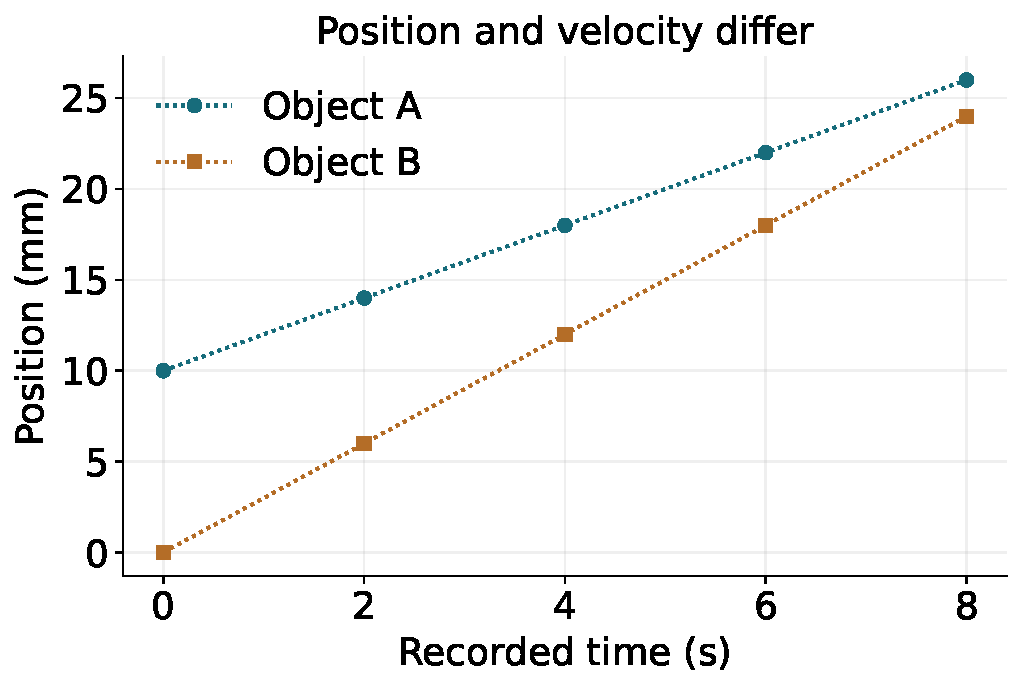
\includegraphics[width=.98\linewidth,height=.69\textheight,keepaspectratio]{position-records.pdf}\end{frame}
\renewcommand{\notestarget}{notes.pdf\#note-translation-of-the-coordinate-origin}
\begin{frame}[t,fragile,label=slide-an-invariance-test]{An invariance test}
\begin{verbatim}
shifted = (26 + 100) - (10 + 100)
assert shifted == 26 - 10
\end{verbatim}
\pause{}
A failed test indicates that the code depends on the origin in a way that the defined statistic does not.
\end{frame}
\renewcommand{\notestarget}{notes.pdf\#note-change-of-physical-units}
\begin{frame}[t,fragile,label=slide-change-of-physical-units]{Change of physical units}
\[
x'=ax,\quad t'=bt\quad\Longrightarrow\quad\overline v'=\frac ab\overline v.
\]
\pause{}
\[
2\ \mathrm{mm/s}=0.2\ \mathrm{cm/s}=12\ \mathrm{cm/min}.
\]
\end{frame}
\renewcommand{\notestarget}{notes.pdf\#note-change-of-physical-units}
\begin{frame}[t,fragile,label=slide-numerical-comparison-after-conversion]{Numerical comparison after conversion}
\begin{verbatim}
dx_mm = 26 - 10
dx_cm = 26/10 - 10/10
assert abs(10*dx_cm - dx_mm) < 1e-12
\end{verbatim}
\pause{}
The tolerance accounts for rounding, not measurement uncertainty.
\end{frame}
\renewcommand{\notestarget}{notes.pdf\#note-displacement-and-path-length}
\begin{frame}[t,fragile,label=slide-displacement-and-path-length]{Displacement and path length}
\[
\Delta x=x_N-x_0=\sum_{i=0}^{N-1}(x_{i+1}-x_i).
\]
\pause{}
\[
|\Delta x|\leq\sum_{i=0}^{N-1}|x_{i+1}-x_i|=L_{\rm sampled}.
\]
\end{frame}
\renewcommand{\notestarget}{notes.pdf\#note-change-of-physical-units}
\begin{frame}[label=slide-displacement-units-figure]{Displacement units}
\centering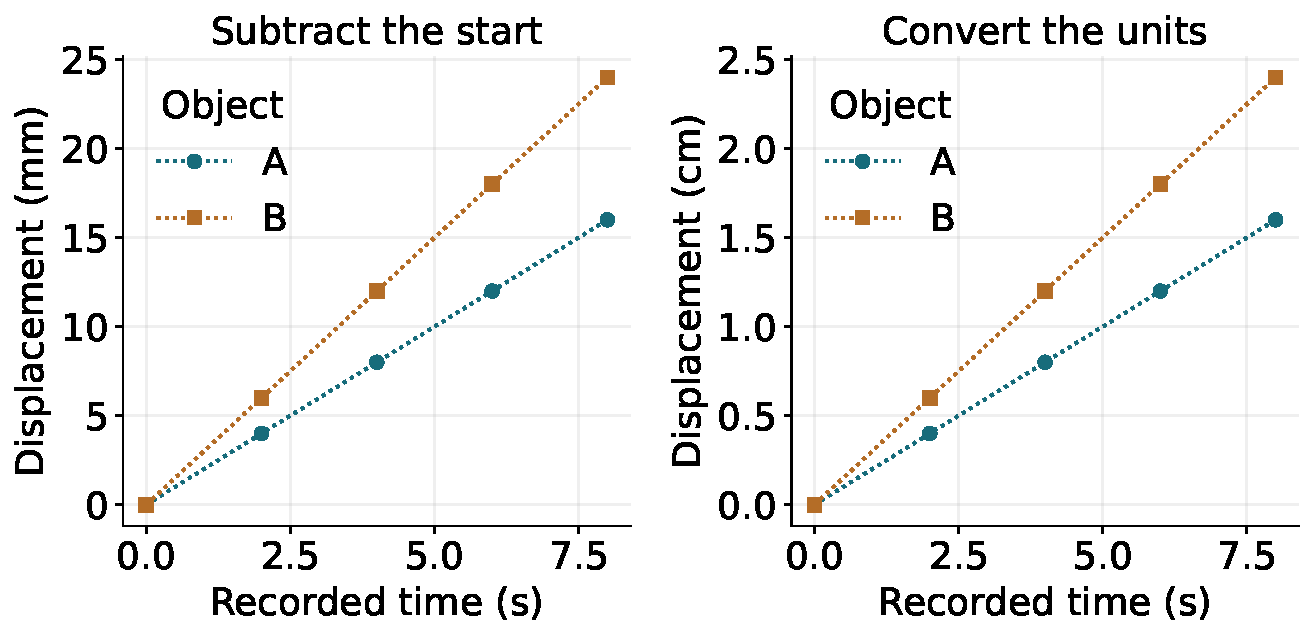
\includegraphics[width=.98\linewidth,height=.69\textheight,keepaspectratio]{displacement-units.pdf}\end{frame}
\renewcommand{\notestarget}{notes.pdf\#note-displacement-and-path-length}
\begin{frame}[t,fragile,label=slide-an-out-and-back-record]{An out-and-back record}
For positions $0,4,0$ at times $0,1,2$,
\[
\Delta x=0,\qquad L_{\rm sampled}=8.
\]
\pause{}
The signed average velocity is zero. The sampled mean speed is $4$ distance units per time unit.
\end{frame}
\renewcommand{\notestarget}{notes.pdf\#note-information-between-samples}
\begin{frame}[t,fragile,label=slide-information-between-samples]{Information between samples}
Two trajectories can agree at every sample time while differing between them.
\pause{}
For a smooth interpolant $x(t)$, add
\[
g(t)=c\prod_i(t-t_i).
\]
The sampled positions stay fixed.
\end{frame}
\renewcommand{\notestarget}{notes.pdf\#note-information-between-samples}
\begin{frame}[t,fragile,label=slide-array-order-and-data-correspondence]{Array order and data correspondence}
\begin{verbatim}
assert len(times_s) == len(a_mm)
plt.plot(times_s, a_mm, "o")
\end{verbatim}
\pause{}
The $i$th time and $i$th position must belong to the same observation. Equal lengths alone do not prove correct pairing.
\end{frame}
\end{document}
